\chapter{数值积分方法}
\section{伽辽金无网格离散控制方程的数值积分方法}
\subsection{高斯积分法}
高斯积分法是指将问题区域离散为一系列背景积分单元$\Omega_C,C=1,2,\dotsb,N\!I\!C$,进行刚度矩阵和力向量的数值积分。高斯积分法的背景网格常采用四边形或三角形网格,如图(\ref{C2GI})所示。
在进行数值时需要将四边形或三角形积分域通过有限元插值函数映射到标准积分单元上具体表达式为:
\begin{equation}
\begin{split}
    \pmb{x}=\sum_{I=1}^{N\!I}N_I(\pmb{\xi})\pmb{x}_I
\end{split}
\end{equation}
其中$N\!I$为背景积分网格节点个数,四边形网格个数为4三角形网格个数为3。$N_I(\pmb{\xi})$为有限元插值函数,四边形背景积分网格表达式为:
\begin{equation}
\begin{split}
    N_I(\pmb{\xi})=\frac{1}{4}(1+\xi_1\xi)(1+\eta_1\eta),I=1,2,3,4
\end{split}
\end{equation}
三角形背景积分网格表达式为:
\begin{equation}
\begin{split}
    N_1(\pmb{\xi})=\xi,N_2(\pmb{\xi})=\eta,N_3(\pmb{\xi})=\zeta=1-\xi-\eta    
\end{split}
\end{equation}\par
对刚度矩阵式(\ref{KIJ})采用高斯积分法得到:
\begin{equation}
\begin{split}
    \pmb{K}_{IJ}&=\int_{\Omega}\pmb{B}_I(\pmb{x})^T\pmb{D}\pmb{B}_J(\pmb{x})d\Omega\\
     &=\sum_{C=1}^{N\!I\!C}\int_{\Omega_C}\pmb{B}_I(\pmb{x})^T\pmb{D}\pmb{B}_J(\pmb{x})d\Omega\\
     &=\sum_{C=1}^{N\!I\!C}\int_{\Omega_C}\int_{-1}^1\int_{-1}^1\pmb{B}_I(\pmb{x})^T\pmb{D}\pmb{B}_J(\pmb{x})Jd\xi d\eta\\
     &=\sum_{C=1}^{N\!I\!C}\sum_{G=1}^{N\!G}\pmb{B}_I(\pmb{x})^T(\pmb{x}_G)\pmb{D}\pmb{B}_J(\pmb{x}_G)J(\pmb{x}_G)\bar{\omega}_G
\end{split}
\end{equation}
其中$N\!G$为每个积分子域积分点的个数,$\pmb{x}_G$为标准单元上高斯点$\pmb{\xi}_G$对应的物理坐标,$\bar{\omega}_G$为积分权重,$J$的具体表达式为:
\begin{equation}
\begin{split}
    J=\vartheta det(\pmb J),\pmb{J}=\frac{\varepsilon\pmb{x}}{\varepsilon\pmb{\xi}}=
    \left[\begin{matrix}
        \frac{\varepsilon x}{\varepsilon\xi}&\frac{\varepsilon x}{\varepsilon\eta}
        \\\frac{\varepsilon y}{\varepsilon\xi}&\frac{\varepsilon y}{\varepsilon\eta}
    \end{matrix}\right]=\sum_{I=1}^{N\!I}
    \left[\begin{matrix}
        \frac{\varepsilon N_I}{\varepsilon\xi}x_I&\frac{\varepsilon N_I}{\varepsilon\eta}x_I
        \\\frac{\varepsilon N_I}{\varepsilon\xi}y_I&\frac{\varepsilon N_I}{\varepsilon\eta}y_I
    \end{matrix}\right]
\end{split}
\end{equation}
式中$\vartheta$为形状参数,四边形网格取为1三角形网格取为0.5。针对三角形网格,雅可比矩阵$\pmb{J}$和其行列式$det(\pmb{J})$存在以下显式表达式:
\begin{equation}
\begin{split}
    &\pmb{J}=\left[\begin{matrix}
       x_2-x_1&x_3-x_1\\y_2-y_1&y_3-y_1
    \end{matrix}\right]\\
&det(\pmb{J})=(x_2-x_1)(y_3-y_1)-(x_3-x_1)(y_2-y_1)
\end{split}
\end{equation}\par
对力向量式(\ref{KIJ})采用高斯积分法可以得到:
\begin{equation}
\begin{split}
   \pmb{f}=\sum_{L=1}^{N\!L}\sum_{B=1}^{N\!B}\Psi_I(\pmb{x}_B)\pmb{g}(\pmb{x}_B)J^B(\pmb{x}_G)\bar{\omega}_B+\sum_{C=1}^{N\!I\!C}\sum_{G=1}^{N\!G}\Psi_I(\pmb{x}_G)\pmb{b}(\pmb{x}_G)J(\pmb{x}_G)\bar{\omega}_G
\end{split}
\end{equation}
其中$\pmb{x}_B$为积分域边界上的积分点,$N\!L$为边界上积分域的个数,$N\!B$为积分域边上的积分点个数。\par
高斯积分法能够在相对较少的积分点上达到较高的精度,适用于光滑函数的积分方法。但在无网格法中应用高斯积分法时,由于无网格形函数本身不是多项式,无法像有限元根据形函数的多项式次数确定采用几个积分点为完全积分,
因此需要注意选择合适的插值方法和插值函数,以及确定适当的积分点数来满足数值积分的精度要求。并且由于高斯积分点不满足积分约束条件,所以一般需要采用高阶高斯积分来保证计算精度,但随着积分点数的增加会导致计算效率的降低。
\begin{figure}[H]
\centering
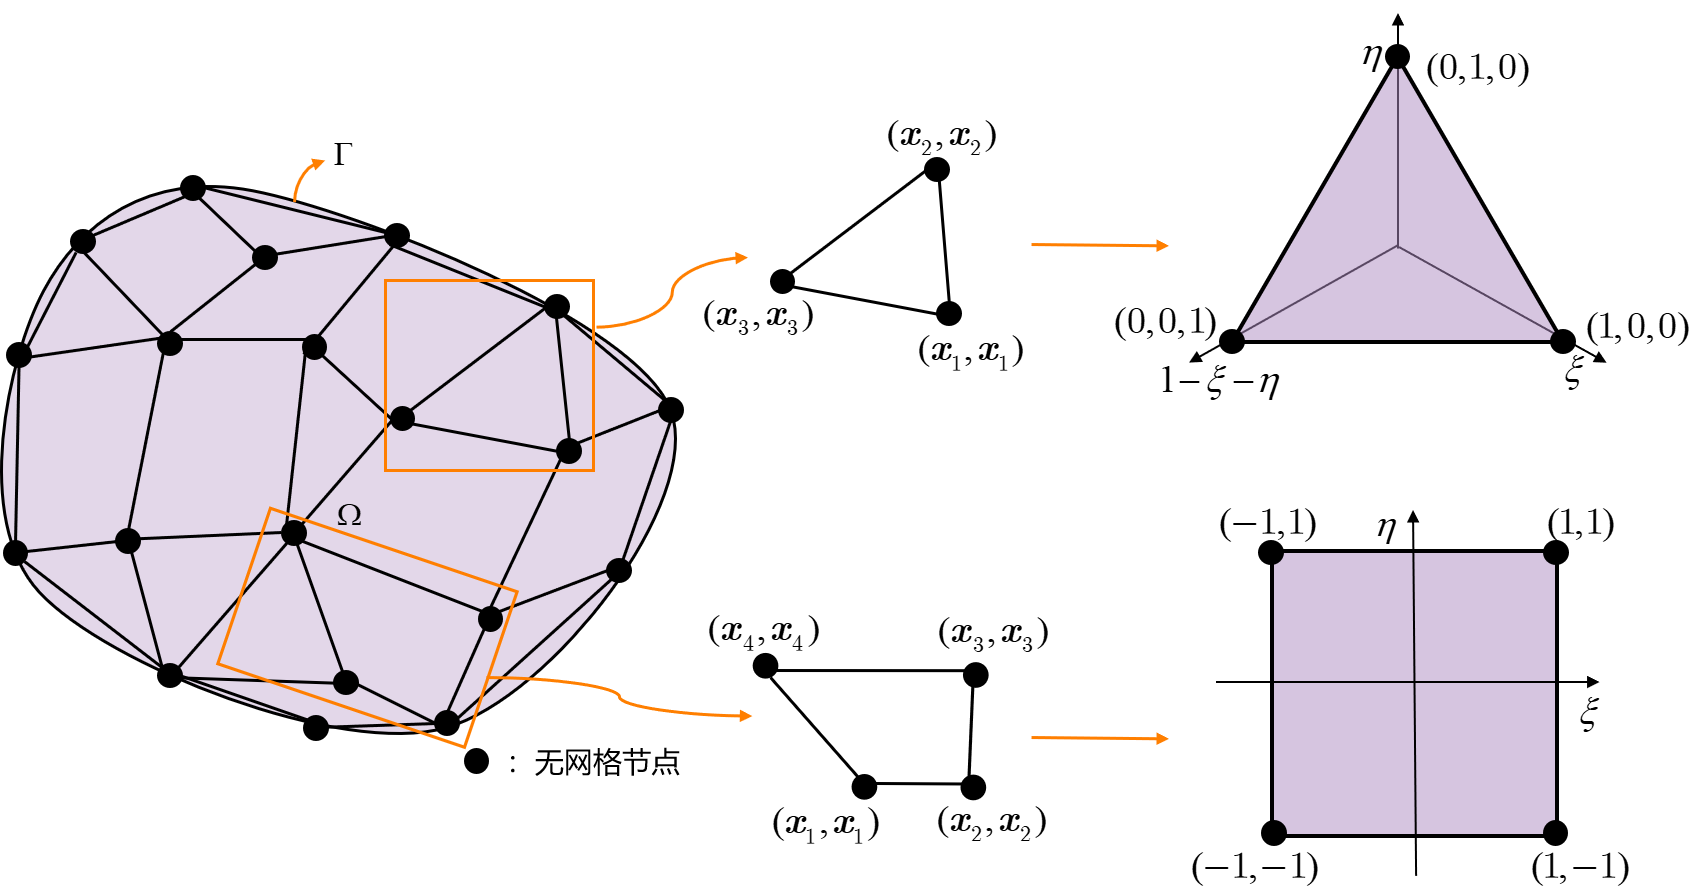
\includegraphics[scale=0.5]{figure/C2/GI.png}
\caption{高斯积分背景网格示意图}\label{C2GI}
\end{figure}
\subsection{再生光滑梯度积分法}
假设场变量$u(\pmb x)$为任意的$p$阶多项式,则其梯度$u_{,i}(\pmb x)$可以表示为:
\begin{equation}
\begin{split}
    u_{,i}(\pmb x)=\pmb a_i^T\pmb q(\pmb x)
\end{split}
\end{equation}
其中$\pmb a_i$表示为任意系数向量;$\pmb q(\pmb x)$为$(p-1)$阶的单项式基向量,即$\pmb q(\pmb x)=\pmb p^{[p-1]}(\pmb x)$,$\pmb{p}(\pmb{x})$是无网格形函数理论中表示$p$阶的多项式基函数向量,根据文献可以知道$(p-1)$阶积分约束条件为:
\begin{equation}\label{p-1}
\begin{split}
    \int_{\Omega}\pmb \Psi_{I,i}\pmb qd\Omega=\int_{\Gamma}\pmb \Psi_I \pmb qn_id\Gamma-\int_{\Omega}\pmb \Psi_I\pmb q_{,i}d\Omega
\end{split}
\end{equation}
根据式子可以看出,由于$p$次基函数,伽辽金弱形式所采用的数值积分方法只有满足$(p-1)$阶积分约束条件,无网格数值解才能重现对应的多项式精确解。\par
根据再生光滑梯度理论,与再生核无网格形函数类似,无网格形函数$\pmb \Psi_I$的再生光滑梯度$\tilde{\pmb\Psi}_{I,i}$可表示为如下形式:
\begin{equation}\label{tildepsi}
\begin{split}
\tilde{\pmb \Psi}_{I,i}(\pmb x)=\pmb q^T(\pmb x)\pmb c_i(\pmb x_I)\tilde{\varphi}(x)
\end{split}
\end{equation}
其中$\pmb c_i$为待定系数向量;$\tilde{\varphi}(\pmb x)$为核函数,这里取为
\begin{equation}
\begin{split}
    \tilde{\varphi}(\pmb x)=\begin{cases}
        1,&\pmb x\in\Omega_c\\
        0,&\pmb x\notin\Omega_c\end{cases}
\end{split}
\end{equation}
其中:$\Omega_C$为互相不重叠且$\cup^{N\!C}_{C=1}\Omega_C=\Omega$的积分单元;
$N\!C$表示的是积分单元的总个数。图(\ref{C2RKGSI})给出了再生光滑梯度无网格法采用采用的三角形背景积分单元。不失为一般性,这里以三次基函数为例详细阐明
再生光滑梯度构造过程。当采用三次基函数$\pmb p(\pmb x)$时,$\pmb q(\pmb x)$的表达式为:
\begin{equation}\label{qx}
\begin{split}
    \pmb q(\pmb x)=(1,x,y,x^2,y^2,xy)^T\quad\pmb x\in\Omega_C
\end{split}
\end{equation}
将式(\ref{qx})代入到积分约束条件式(\ref{p-1})中,可得到:
\begin{equation}\label{tildegc}
\begin{split}
    \int_{\Omega_C}\pmb \Psi_{I,i}\pmb qd\Omega=\tilde{\pmb g}^C_{iI},I=1,2,\dotsb,N\!P
\end{split}
\end{equation}
\begin{equation}
\begin{split}
     \tilde{\pmb g}^C_{iI}=\int_{\Gamma_C}\pmb \Psi_I\pmb qn_id\Gamma-\int_{\Omega_C}\pmb \Psi_I\pmb q_{,i}d\Omega
    \end{split}
\end{equation}
再用式子(\ref{tildepsi})定义的光滑梯度$\tilde{\pmb \Psi}_{I,i}$替换到式子(\ref{tildegc})中的标准梯度$\pmb \Psi_{I,i}$,可以得到$\pmb c_i=\pmb G^{-1}_C\:\tilde{\pmb g}^C_{iI}$
其中$\pmb G_C$为再生光滑梯度的矩量矩阵,其表达式为:
\begin{equation}\label{GC}
\begin{split}
    \pmb G_C=\int_{\Omega_C}\pmb q\pmb q^Td\Omega
\end{split}
\end{equation}
如图(\ref{C2RKGSI})所示,为了方便数值积分再生光滑梯度积分法将三角形积分域投影至参数空间。在投影后的三角形积分域内采用高斯积分法求解得到$\tilde{\pmb g}_{iI}^C$,具体表达式为:
\begin{equation}\label{tildegciI}
\begin{split}
    \tilde{\pmb{g}}_{iI}^C&=\sum_{C=1}^{N\!C}\sum_{G\!B=\mathbb{A}(\Gamma_C)}\Psi_I(\pmb{x}_{GB})\pmb{q}(\pmb{x}_{GB})\pmb{n}_i\pmb{J}(\pmb{x}_{GB})\omega_{GB}\\
    &-\sum_{C=1}^{N\!C}\sum_{G\!I=\mathbb{A}(\Omega_C)}\Psi_I(x_{GI})q_{,i}(x_{GI})J(x_{GI})\omega_{GI}
\end{split}
\end{equation}
其中$\mathbb{A}$为背景积分单元内部或者边界上的高斯积分点总数量;$\pmb{x}_{GB}$、$\pmb{\omega_{GB}}$表示背景积分单元边界上的高斯积分点位置和相应的权重;
$x_{GI}$、$\omega_{GI}$为背景积分单元内的高斯积分点位置与配套的权重;$\pmb{J}$表示背景积分单元联系物理和参数空间的雅可比矩阵行列式。
值得注意的是式(\ref{GC})中的$\pmb{G}_C$不需要采用数值积分计算可以直接解析得到。\par
根据式(\ref{tildepsi})和式(\ref{tildegciI}),可以得到背景积分域内的再生光滑梯度积分表达式为:
\begin{equation}\label{ftildepsi}
\begin{split}
    \tilde{\Psi}_{I,i}(\pmb{x})=\pmb{q}^T(\pmb{x})\pmb{G}^{-1}_C\tilde{g}^C_{iI},\~x\in\Omega_C
\end{split}
\end{equation}
根据式(\ref{ftildepsi})可以看出再生光滑梯度通过直接构造得到,避免了标准无网格梯度的复杂计算,有效的提高了计算精度和计算效率。值得注意的是,再生光滑梯度仅用于刚度矩阵的构造,
对于弹性力学问题中的应力和应变计算,仍然采用传统的无网格形函数及梯度的构造。这是由于再生光滑梯度并非全域连续函数,是在局部背景积分域内满足积分约束条件进而在全域上满足积分约束条件。
\begin{figure}[H]
\centering
    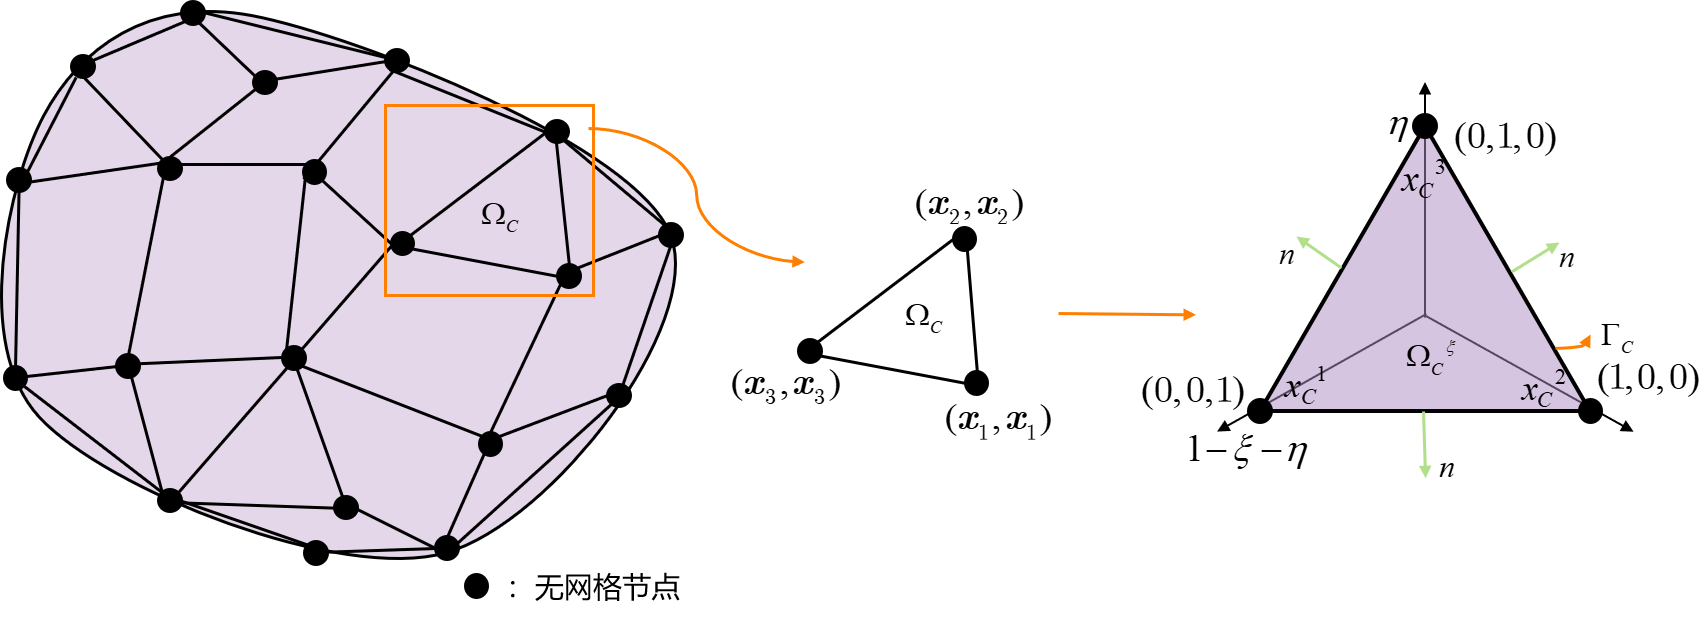
\includegraphics[scale=0.5]{figure/C2/RKGSI.png}
    \caption{三角形背景积分单元示意图}\label{C2RKGSI}
\end{figure}
